\documentclass[10pt,letterpaper]{article}
\usepackage{aaai}
\usepackage{xparse}
\usepackage{times}
\usepackage{helvet}
\usepackage{courier}

\usepackage{amsmath}
\usepackage{amssymb}
\usepackage{xspace}
\usepackage{relsize}
\usepackage{aaai_my}
\usepackage{graphicx}
\usepackage{abbrev}
\usepackage{multirow}
\usepackage{xr}
\externaldocument{asai}
\renewcommand{\thetable}{S\arabic{table}}
\renewcommand{\thefigure}{S\arabic{figure}}

\setlength{\pdfpagewidth}{8.5in}
\setlength{\pdfpageheight}{11in}
\pagestyle{empty}
\frenchspacing
% \setlength{\floatsep}{1mm}
% \setlength{\textfloatsep}{1mm}
% \setlength{\abovecaptionskip}{1mm}
% \setlength{\belowcaptionskip}{1mm}
% \setlength{\abovedisplayskip}{1mm}
% \setlength{\belowdisplayskip}{1mm}
% \setlength{\arraycolsep}{0.5mm}
\setlength{\tabcolsep}{0.1em}

\nocopyright
\author{Submision 974}
\title{Tiebreaking Strategies for Classical Planning Using $A^*$ Search\\ (Supplemental Material)}
\begin{document}
\maketitle

\section{\refig{plateau-noh-full}: Colored, fully labeled version of \refig{fig:plateau-noh}}

\begin{figure}[hb]
 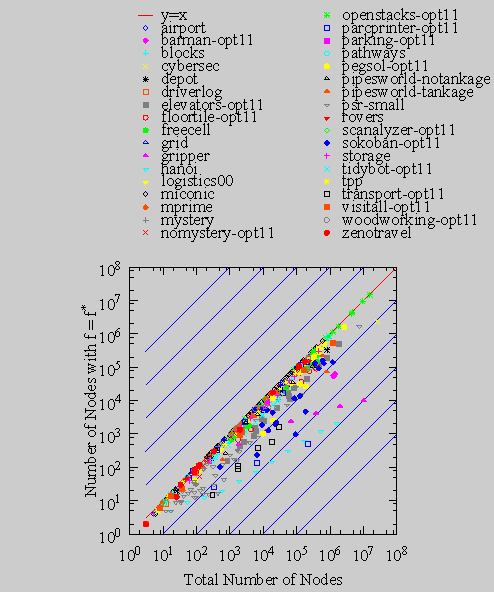
\includegraphics{tables/aaai16-frontier/aaai16prelim3/lmcut_frontier_noh-front.pdf}
 \caption{
 The number of nodes with $f=f^*$ (y-axis) compared to the
 total number of nodes in the search space (x-axis) with $f\leq f^*$
 on 1104 IPC benchmark problems,
 using a modified Fast Downward (with \lmcut) which 
 generates all nodes $f\leq f^*$.
 Blue lines are $y=x \times 10^n$ for $n=\pm1,\pm2,\cdots$.
 Many instances belongs to the region $y>x/10$.
 }
 \label{plateau-noh-full}
\end{figure}

\newpage

\section{\refig{plateau-full}: Colored, fully labeled version of \refig{plateau}}


\begin{figure}[htb]
 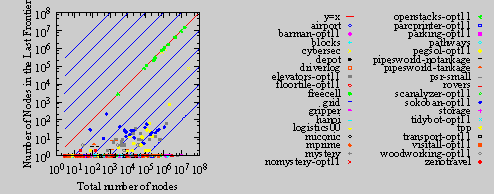
\includegraphics{tables/aaai16-frontier/aaai16prelim3/lmcut_frontier-front.pdf}
 \caption{
 Similar to \refig{plateau-noh-full}; $y$-axis shows
 number of nodes with $f=f^*, h=0$, which forms the final
  plateau when $h$-based tie-breaking is enabled.
  Note that many \pddl{Openstacks} and \pddl{Cybersec} instances are near the $y=x$ line.
  %Due to space, we do not show all labels for point types. 
 }
 \label{plateau-full}
\end{figure}

\newpage
\section{\refig{plateau-zerocost-full}: Colored, fully labeled version of \refig{plateau-zerocost}}

\begin{figure}[htb]
 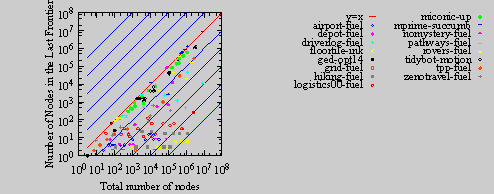
\includegraphics{tables/aaai16-frontier/zerocost/lmcut_frontier-front.pdf}
 \caption{Similar to \refig{plateau}, but for 620 instances from our 
 \emph{zerocost domains} (\refsec{sec:zerocost-domains}),
 where zero-cost actions induce very large plateaus.
 Even with $h$ tie-breaking, these domains force the planner
 to search much larger plateau.
 }
 \label{plateau-zerocost-full}
\end{figure}

\newpage
\section{\refig{f-h-eval-full}: Colored, fully labeled version of \refig{f-h-eval}}

\begin{figure}[htb]
 \centering \relsize{-3}
 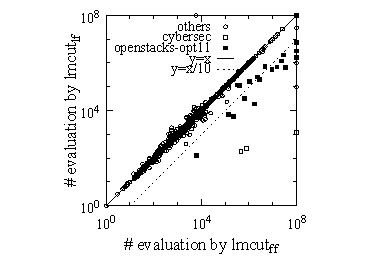
\includegraphics{tables/aaai16-30min-5min-cut/aaai16prelim3/evaluated-lmcut_ff-lmcut_lf.pdf}
 \caption{Comparisons of the number evaluations between simple \lifo and
 \fifo second-level tie-breaking, with first-level $h$
 tie-breaking. \lifo evaluates less than $1/10$ of the nodes evaluated
 by \fifo in Cybersec and Openstacks.}
 \label{f-h-eval-full}
\end{figure}

\clearpage
\onecolumn
\section{Full Tables for \reftbl{depth} : Part 1, IPC domains, \lmcut}

\begin{table*}[htb]
 {
 \centering
 \begin{tabular}{|c|c|c|c|c|c|c|c|c|c|c|c|c|}
\hline
 & \multicolumn{4}{|c|}{Coverages}
 & \multicolumn{5}{|c||}{Coverages (mean$\pm$sd)}
 & \multicolumn{3}{|c|}{Wilcoxon $p$ vs $[h,\rd,\ro]$} \\
\hline                                    
 Domain &  $[h,\fifo]$ &  $[h,\lifo]$ &  $[\fifo]$ &  $[\lifo]$ &  $[h,\fd,\ro]$ &  $[h,\ld,\ro]$ &  $[h,\rd,\ro]$ &  $[\rd,\ro]$ &  $[h,\ro]$ & $[h,\fd,\ro]$   & $[h,\ld,\ro]$   & $[h,\ro]$    \\
\hline                                    
 sum(1104)&558&565&442&556&554.6\spm{}0.8&568.3\spm{}1.8&\textbf{570.6\spm{}1.5}&560.0\spm{}0.9&559.8\spm{}1.0&\textbf{0.0}&\textbf{.01}&\textbf{0.0}  \\
\hline                                    
 {\relsize{-1}airport(50)}&\textbf{27}&26&18&26&25.6\spm{}0.5&25.8\spm{}0.6&25.9\spm{}0.5&21.0\spm{}0.0&26.0\spm{}0.0&.26&.72&.58  \\
 {\relsize{-1}barman-opt11(20)}&0&0&0&0&0.0\spm{}0.0&0.0\spm{}0.0&0.0\spm{}0.0&0.0\spm{}0.0&0.0\spm{}0.0&1.0&1.0&1.0  \\
 {\relsize{-1}blocks(35)}&28&28&26&26&28.0\spm{}0.0&28.0\spm{}0.0&28.0\spm{}0.0&27.0\spm{}0.0&28.0\spm{}0.0&1.0&1.0&1.0  \\
 {\relsize{-1}cybersec(19)}&2&3&0&3&2.0\spm{}0.0&7.3\spm{}1.5&\textbf{9.6\spm{}1.1}&7.8\spm{}0.7&4.4\spm{}1.0&\textbf{0.0}&\textbf{.01}&\textbf{0.0}  \\
 {\relsize{-1}depot(22)}&6&6&5&5&6.0\spm{}0.0&6.0\spm{}0.0&6.0\spm{}0.0&6.0\spm{}0.0&6.0\spm{}0.0&1.0&1.0&1.0  \\
 {\relsize{-1}driverlog(20)}&13&13&12&13&13.0\spm{}0.0&13.0\spm{}0.0&13.0\spm{}0.0&13.0\spm{}0.0&13.0\spm{}0.0&1.0&1.0&1.0  \\
 {\relsize{-1}elevators-opt11(20)}&15&15&14&15&15.0\spm{}0.0&15.0\spm{}0.0&15.0\spm{}0.0&14.8\spm{}0.4&15.0\spm{}0.0&1.0&1.0&1.0  \\
 {\relsize{-1}floortile-opt11(20)}&6&6&6&6&6.0\spm{}0.0&6.0\spm{}0.0&6.0\spm{}0.0&6.0\spm{}0.0&6.0\spm{}0.0&1.0&1.0&1.0  \\
 {\relsize{-1}freecell(80)}&9&9&8&9&9.0\spm{}0.0&9.0\spm{}0.0&9.0\spm{}0.0&9.0\spm{}0.0&9.0\spm{}0.0&1.0&1.0&1.0  \\
 {\relsize{-1}grid(5)}&1&1&1&1&1.0\spm{}0.0&1.0\spm{}0.0&1.0\spm{}0.0&1.0\spm{}0.0&1.0\spm{}0.0&1.0&1.0&1.0  \\
 {\relsize{-1}gripper(20)}&6&6&6&6&6.0\spm{}0.0&6.0\spm{}0.0&6.0\spm{}0.0&6.0\spm{}0.0&6.0\spm{}0.0&1.0&1.0&1.0  \\
 {\relsize{-1}hanoi(30)}&12&12&12&12&12.0\spm{}0.0&12.0\spm{}0.0&12.0\spm{}0.0&12.0\spm{}0.0&12.0\spm{}0.0&1.0&1.0&1.0  \\
 {\relsize{-1}logistics00(28)}&\textbf{20}&\textbf{20}&16&18&\textbf{20.0\spm{}0.0}&\textbf{20.0\spm{}0.0}&\textbf{20.0\spm{}0.0}&\textbf{20.0\spm{}0.0}&\textbf{20.0\spm{}0.0}&1.0&1.0&1.0  \\
 {\relsize{-1}miconic(150)}&\textbf{140}&\textbf{140}&68&\textbf{140}&\textbf{140.0\spm{}0.0}&\textbf{140.0\spm{}0.0}&\textbf{140.0\spm{}0.0}&135.6\spm{}0.5&\textbf{140.0\spm{}0.0}&1.0&1.0&1.0  \\
 {\relsize{-1}mprime(35)}&21&21&19&22&20.9\spm{}0.3&20.9\spm{}0.3&20.9\spm{}0.3&21.0\spm{}0.0&20.9\spm{}0.3&1.0&1.0&1.0  \\
 {\relsize{-1}mystery(30)}&15&16&15&15&15.0\spm{}0.0&15.0\spm{}0.0&15.0\spm{}0.0&15.8\spm{}0.4&15.0\spm{}0.0&1.0&1.0&1.0  \\
 {\relsize{-1}nomystery-opt11(20)}&14&14&12&13&14.0\spm{}0.0&14.0\spm{}0.0&14.0\spm{}0.0&13.8\spm{}0.4&14.0\spm{}0.0&1.0&1.0&1.0  \\
 {\relsize{-1}openstacks-opt11(20)}&11&\textbf{18}&11&\textbf{18}&10.0\spm{}0.0&\textbf{18.0\spm{}0.0}&\textbf{18.0\spm{}0.0}&\textbf{18.0\spm{}0.0}&11.6\spm{}0.5&\textbf{0.0}&1.0&\textbf{0.0}  \\
 {\relsize{-1}parcprinter-opt11(20)}&13&13&12&13&13.0\spm{}0.0&13.0\spm{}0.0&13.0\spm{}0.0&13.0\spm{}0.0&13.0\spm{}0.0&1.0&1.0&1.0  \\
 {\relsize{-1}parking-opt11(20)}&1&1&1&1&1.0\spm{}0.0&1.0\spm{}0.0&1.0\spm{}0.0&1.0\spm{}0.0&1.0\spm{}0.0&1.0&1.0&1.0  \\
 {\relsize{-1}pathways(30)}&5&5&4&5&5.0\spm{}0.0&5.0\spm{}0.0&5.0\spm{}0.0&5.0\spm{}0.0&5.0\spm{}0.0&1.0&1.0&1.0  \\
 {\relsize{-1}pegsol-opt11(20)}&17&17&17&17&17.0\spm{}0.0&17.0\spm{}0.0&17.0\spm{}0.0&17.0\spm{}0.0&17.0\spm{}0.0&1.0&1.0&1.0  \\
 {\relsize{-1}pipesworld-notankage(50)}&15&14&13&13&14.1\spm{}0.3&14.3\spm{}0.5&14.2\spm{}0.4&14.2\spm{}0.4&14.9\spm{}0.3&.58&.65&\textbf{0.0}  \\
 {\relsize{-1}pipesworld-tankage(50)}&8&8&7&8&8.0\spm{}0.0&8.0\spm{}0.0&8.0\spm{}0.0&8.0\spm{}0.0&8.0\spm{}0.0&1.0&1.0&1.0  \\
 {\relsize{-1}psr-small(50)}&48&48&48&48&48.0\spm{}0.0&48.0\spm{}0.0&48.0\spm{}0.0&48.0\spm{}0.0&48.0\spm{}0.0&1.0&1.0&1.0  \\
 {\relsize{-1}rovers(40)}&7&7&7&7&7.0\spm{}0.0&7.0\spm{}0.0&7.0\spm{}0.0&7.0\spm{}0.0&7.0\spm{}0.0&1.0&1.0&1.0  \\
 {\relsize{-1}scanalyzer-opt11(20)}&\textbf{10}&\textbf{10}&4&\textbf{10}&\textbf{10.0\spm{}0.0}&\textbf{10.0\spm{}0.0}&\textbf{10.0\spm{}0.0}&9.0\spm{}0.0&\textbf{10.0\spm{}0.0}&1.0&1.0&1.0  \\
 {\relsize{-1}sokoban-opt11(20)}&19&19&19&19&19.0\spm{}0.0&19.0\spm{}0.0&19.0\spm{}0.0&19.0\spm{}0.0&19.0\spm{}0.0&1.0&1.0&1.0  \\
 {\relsize{-1}storage(30)}&14&14&14&14&14.0\spm{}0.0&14.0\spm{}0.0&14.0\spm{}0.0&14.4\spm{}0.5&14.0\spm{}0.0&1.0&1.0&1.0  \\
 {\relsize{-1}tidybot-opt11(20)}&12&12&11&11&12.0\spm{}0.0&12.0\spm{}0.0&12.0\spm{}0.0&11.8\spm{}0.4&12.0\spm{}0.0&1.0&1.0&1.0  \\
 {\relsize{-1}tpp(30)}&6&6&6&6&6.0\spm{}0.0&6.0\spm{}0.0&6.0\spm{}0.0&6.0\spm{}0.0&6.0\spm{}0.0&1.0&1.0&1.0  \\
 {\relsize{-1}transport-opt11(20)}&6&6&6&6&6.0\spm{}0.0&6.0\spm{}0.0&6.0\spm{}0.0&6.0\spm{}0.0&6.0\spm{}0.0&1.0&1.0&1.0  \\
 {\relsize{-1}visitall-opt11(20)}&10&10&9&10&10.0\spm{}0.0&10.0\spm{}0.0&10.0\spm{}0.0&10.0\spm{}0.0&10.0\spm{}0.0&1.0&1.0&1.0  \\
 {\relsize{-1}woodworking-opt11(20)}&10&10&6&9&10.0\spm{}0.0&10.0\spm{}0.0&10.0\spm{}0.0&\textbf{11.8\spm{}0.4}&10.0\spm{}0.0&1.0&1.0&1.0  \\
 {\relsize{-1}zenotravel(20)}&11&11&9&11&11.0\spm{}0.0&11.0\spm{}0.0&11.0\spm{}0.0&11.0\spm{}0.0&11.0\spm{}0.0&1.0&1.0&1.0 \\\hline
\end{tabular}

 \caption{
 Full version of the upper half of \reftbl{depth} showing 
 the experiments on the IPC benchmark instances.
 Each cell shows the coverage of the domain solved with 5 min, 2GB,
 using \lmcut heuritics.
 }
 \label{lmcut-ipc-full}
 }
\end{table*}

\newpage
\section{Full Tables for \reftbl{depth} : Part 2, Zerocost domains, \lmcut}

\begin{table*}[htb]
 {
 \centering
 \begin{tabular}{|c|c|c|c|c|c|c|c|c|c|c|c|c|}
\hline
 & \multicolumn{4}{|c|}{Coverages}
 & \multicolumn{5}{|c||}{Coverages (mean$\pm$sd)}
 & \multicolumn{3}{|c|}{Wilcoxon $p$ vs $[h,\rd,\ro]$} \\
\hline                                    
 Domain &  $[h,\fifo]$ &  $[h,\lifo]$ &  $[\fifo]$ &  $[\lifo]$ &  $[h,\fd,\ro]$ &  $[h,\ld,\ro]$ &  $[h,\rd,\ro]$ &  $[\rd,\ro]$ &  $[h,\ro]$ & $[h,\fd,\ro]$   & $[h,\ld,\ro]$   & $[h,\ro]$    \\
\hline                                    
 sum(620)&256&279&212&281&249.1\spm{}1.8&280.2\spm{}7.9&287.2\spm{}2.4&280.2\spm{}4.2&264.9\spm{}1.8&\textbf{0.0}&\textbf{.02}&\textbf{0.0}  \\
\hline                                    
 {\relsize{-1}airport-fuel(20)}&15&13&7&15&14.2\spm{}0.9&13.8\spm{}0.6&14.4\spm{}0.7&10.4\spm{}0.5&14.4\spm{}0.7&.49&.06&1.0  \\
 {\relsize{-1}blocks-stack(20)}&17&17&15&17&17.0\spm{}0.0&17.1\spm{}0.3&17.0\spm{}0.0&16.0\spm{}0.0&17.0\spm{}0.0&1.0&.37&1.0  \\
 {\relsize{-1}depot-fuel(22)}&6&6&4&6&6.0\spm{}0.0&6.0\spm{}0.0&6.0\spm{}0.0&6.0\spm{}0.0&6.0\spm{}0.0&1.0&1.0&1.0  \\
 {\relsize{-1}driverlog-fuel(20)}&8&8&7&8&8.0\spm{}0.0&7.2\spm{}0.7&8.0\spm{}0.0&8.0\spm{}0.0&8.0\spm{}0.0&1.0&\textbf{.01}&1.0  \\
 {\relsize{-1}elevators-up(20)}&7&13&7&13&5.3\spm{}0.5&8.8\spm{}0.9&9.4\spm{}1.1&8.2\spm{}0.7&7.3\spm{}0.5&\textbf{0.0}&.25&\textbf{0.0}  \\
 {\relsize{-1}floortile-ink(20)}&8&8&8&8&8.0\spm{}0.0&8.0\spm{}0.0&8.1\spm{}0.3&8.0\spm{}0.0&8.3\spm{}0.5&.37&.37&0.3  \\
 {\relsize{-1}freecell-move(20)}&4&19&4&19&4.0\spm{}0.0&19.4\spm{}0.5&16.5\spm{}0.7&16.6\spm{}0.8&5.0\spm{}0.4&\textbf{0.0}&\textbf{0.0}&\textbf{0.0}  \\
 {\relsize{-1}grid-fuel(5)}&1&1&1&1&1.0\spm{}0.0&1.0\spm{}0.0&1.0\spm{}0.0&1.0\spm{}0.0&1.0\spm{}0.0&1.0&1.0&1.0  \\
 {\relsize{-1}gripper-move(20)}&7&7&7&7&6.0\spm{}0.0&6.0\spm{}0.0&6.0\spm{}0.0&7.0\spm{}0.0&7.0\spm{}0.0&1.0&1.0&\textbf{0.0}  \\
 {\relsize{-1}hiking-fuel(20)}&9&9&8&9&9.0\spm{}0.0&9.0\spm{}0.0&9.0\spm{}0.0&9.0\spm{}0.0&9.0\spm{}0.0&1.0&1.0&1.0  \\
 {\relsize{-1}logistics00-fuel(28)}&16&16&15&16&15.0\spm{}0.0&15.0\spm{}0.0&15.0\spm{}0.0&16.0\spm{}0.0&16.0\spm{}0.0&1.0&1.0&\textbf{0.0}  \\
 {\relsize{-1}miconic-up(30)}&16&17&10&17&15.4\spm{}0.5&18.0\spm{}1.3&19.8\spm{}1.0&20.4\spm{}1.0&17.0\spm{}0.4&\textbf{0.0}&\textbf{0.0}&\textbf{0.0}  \\
 {\relsize{-1}mprime-succumb(35)}&15&14&12&14&15.8\spm{}0.7&18.7\spm{}3.9&20.1\spm{}0.7&18.6\spm{}2.0&17.9\spm{}0.5&\textbf{0.0}&.23&\textbf{0.0}  \\
 {\relsize{-1}mystery-feast(20)}&7&5&5&5&7.2\spm{}0.4&6.2\spm{}0.7&7.2\spm{}0.4&7.2\spm{}0.7&7.3\spm{}0.5&1.0&\textbf{0.0}&.65  \\
 {\relsize{-1}nomystery-fuel(20)}&10&10&9&10&10.0\spm{}0.0&10.0\spm{}0.0&10.0\spm{}0.0&9.4\spm{}0.5&10.0\spm{}0.0&1.0&1.0&1.0  \\
 {\relsize{-1}parking-movecc(20)}&0&0&0&0&0.0\spm{}0.0&0.0\spm{}0.0&0.0\spm{}0.0&0.0\spm{}0.0&0.0\spm{}0.0&1.0&1.0&1.0  \\
 {\relsize{-1}pathways-fuel(30)}&5&5&4&5&4.0\spm{}0.0&4.2\spm{}0.4&4.4\spm{}0.5&4.8\spm{}0.4&4.4\spm{}0.5&\textbf{.03}&.37&1.0  \\
 {\relsize{-1}pipesnt-pushstart(20)}&8&8&6&7&8.0\spm{}0.0&8.6\spm{}1.3&9.8\spm{}0.4&9.8\spm{}0.4&8.5\spm{}0.5&\textbf{0.0}&\textbf{.04}&\textbf{0.0}  \\
 {\relsize{-1}pipesworld-pushend(20)}&3&4&2&4&3.0\spm{}0.0&4.2\spm{}1.0&4.5\spm{}0.8&5.4\spm{}0.8&3.9\spm{}0.3&\textbf{0.0}&0.5&\textbf{.05}  \\
 {\relsize{-1}psr-small-open(20)}&19&19&19&19&18.0\spm{}0.0&19.0\spm{}0.0&19.0\spm{}0.0&19.0\spm{}0.0&19.0\spm{}0.0&\textbf{0.0}&1.0&1.0  \\
 {\relsize{-1}rovers-fuel(40)}&8&8&7&9&8.0\spm{}0.0&8.0\spm{}0.0&8.0\spm{}0.0&9.0\spm{}0.0&8.0\spm{}0.0&1.0&1.0&1.0  \\
 {\relsize{-1}scanalyzer-analyze(20)}&9&9&3&9&9.7\spm{}0.6&9.3\spm{}0.5&9.1\spm{}0.3&7.4\spm{}1.0&9.1\spm{}0.3&\textbf{.02}&0.3&1.0  \\
 {\relsize{-1}sokoban-pushgoal(20)}&18&18&18&18&18.0\spm{}0.0&17.0\spm{}0.0&17.9\spm{}0.3&17.0\spm{}0.0&18.0\spm{}0.0&.37&\textbf{0.0}&.37  \\
 {\relsize{-1}storage-lift(20)}&4&4&4&4&4.0\spm{}0.0&5.0\spm{}1.2&4.4\spm{}0.5&4.6\spm{}0.5&4.6\spm{}0.5&\textbf{.03}&.26&.41  \\
 {\relsize{-1}tidybot-motion(20)}&16&16&14&16&16.0\spm{}0.0&16.0\spm{}0.0&16.0\spm{}0.0&15.6\spm{}0.5&16.0\spm{}0.0&1.0&1.0&1.0  \\
 {\relsize{-1}tpp-fuel(30)}&8&11&7&11&7.0\spm{}0.0&11.0\spm{}0.0&11.0\spm{}0.0&11.0\spm{}0.0&8.1\spm{}0.3&\textbf{0.0}&1.0&\textbf{0.0}  \\
 {\relsize{-1}woodworking-cut(20)}&5&7&2&7&4.5\spm{}0.5&6.7\spm{}0.5&8.6\spm{}0.9&7.8\spm{}0.7&7.1\spm{}0.3&\textbf{0.0}&\textbf{0.0}&\textbf{0.0}  \\
 {\relsize{-1}zenotravel-fuel(20)}&7&7&7&7&7.0\spm{}0.0&7.0\spm{}0.0&7.0\spm{}0.0&7.0\spm{}0.0&7.0\spm{}0.0&1.0&1.0&1.0 \\\hline
\end{tabular}

 \caption{
 Full version of the upper half of \reftbl{depth} showing 
 the experiments on the Zerocost instances.
 Each cell shows the coverage of the domain solved with 5 min, 2GB,
 using \lmcut heuritics.
 }
 \label{lmcut-zerocost-full}
 }
\end{table*}

\newpage
\section{Full Tables for \reftbl{depth} : Part 3, IPC domains, \mands}

\begin{table*}[htb]
 {
 \centering
 \begin{tabular}{|c|c|c|c|c|c|c|c|c|c|c|c|c|}
\hline                                    
 & \multicolumn{4}{|c|}{Coverages}
 & \multicolumn{5}{|c||}{Coverages (mean$\pm$sd)}
 & \multicolumn{3}{|c|}{Wilcoxon $p$ vs $[h,\rd,\ro]$} \\
\hline                                    
 Domain &  $[h,\fifo]$ &  $[h,\lifo]$ &  $[\fifo]$ &  $[\lifo]$ &  $[h,\fd,\ro]$ &  $[h,\ld,\ro]$ &  $[h,\rd,\ro]$ &  $[\rd,\ro]$ &  $[h,\ro]$ & $[h,\fd,\ro]$   & $[h,\ld,\ro]$   & $[h,\ro]$    \\
\hline                                    
 sum(1104) &  479 &  488 &  451 &  481 &  478.8\spm{}0.4 &  484.8\spm{}0.4 &  484.0\spm{}0.0 &  481.4\spm{}1.4 &  486.4\spm{}0.8 &  \textbf{.01} &  \textbf{.02} &  \textbf{.01}  \\
\hline                                    
 {\relsize{-1}airport(50)} &  9 &  9 &  9 &  8 &  9.0\spm{}0.0 &  9.0\spm{}0.0 &  9.0\spm{}0.0 &  9.0\spm{}0.0 &  9.0\spm{}0.0 &  1.0 &  1.0 &  1.0  \\
 {\relsize{-1}barman-opt11(20)} &  4 &  4 &  4 &  4 &  4.0\spm{}0.0 &  4.0\spm{}0.0 &  4.0\spm{}0.0 &  4.0\spm{}0.0 &  4.0\spm{}0.0 &  1.0 &  1.0 &  1.0  \\
 {\relsize{-1}blocks(35)} &  22 &  21 &  21 &  21 &  21.6\spm{}0.5 &  21.6\spm{}0.5 &  21.6\spm{}0.5 &  21.8\spm{}0.4 &  22.0\spm{}0.0 &  1.0 &  1.0 &  .18  \\
 {\relsize{-1}cybersec(19)} &  0 &  0 &  0 &  0 &  0.0\spm{}0.0 &  0.0\spm{}0.0 &  0.0\spm{}0.0 &  0.0\spm{}0.0 &  0.0\spm{}0.0 &  1.0 &  1.0 &  1.0  \\
 {\relsize{-1}depot(22)} &  5 &  6 &  5 &  5 &  5.0\spm{}0.0 &  5.0\spm{}0.0 &  5.0\spm{}0.0 &  5.0\spm{}0.0 &  5.0\spm{}0.0 &  1.0 &  1.0 &  1.0  \\
 {\relsize{-1}driverlog(20)} &  12 &  12 &  11 &  12 &  12.0\spm{}0.0 &  12.0\spm{}0.0 &  12.0\spm{}0.0 &  12.0\spm{}0.0 &  12.0\spm{}0.0 &  1.0 &  1.0 &  1.0  \\
 {\relsize{-1}elevators-opt11(20)} &  12 &  12 &  11 &  11 &  12.0\spm{}0.0 &  12.0\spm{}0.0 &  12.0\spm{}0.0 &  12.0\spm{}0.0 &  13.0\spm{}0.0 &  1.0 &  1.0 &  \textbf{0.0}  \\
 {\relsize{-1}floortile-opt11(20)} &  6 &  6 &  5 &  5 &  6.0\spm{}0.0 &  6.0\spm{}0.0 &  6.0\spm{}0.0 &  5.2\spm{}0.4 &  6.0\spm{}0.0 &  1.0 &  1.0 &  1.0  \\
 {\relsize{-1}freecell(80)} &  17 &  17 &  15 &  16 &  16.0\spm{}0.0 &  16.0\spm{}0.0 &  16.0\spm{}0.0 &  15.6\spm{}0.5 &  16.0\spm{}0.0 &  1.0 &  1.0 &  1.0  \\
 {\relsize{-1}grid(5)} &  2 &  2 &  2 &  2 &  2.0\spm{}0.0 &  2.0\spm{}0.0 &  2.0\spm{}0.0 &  2.0\spm{}0.0 &  2.0\spm{}0.0 &  1.0 &  1.0 &  1.0  \\
 {\relsize{-1}gripper(20)} &  20 &  20 &  7 &  20 &  20.0\spm{}0.0 &  20.0\spm{}0.0 &  20.0\spm{}0.0 &  20.0\spm{}0.0 &  20.0\spm{}0.0 &  1.0 &  1.0 &  1.0  \\
 {\relsize{-1}hanoi(30)} &  14 &  14 &  14 &  14 &  14.0\spm{}0.0 &  14.0\spm{}0.0 &  14.0\spm{}0.0 &  14.0\spm{}0.0 &  14.0\spm{}0.0 &  1.0 &  1.0 &  1.0  \\
 {\relsize{-1}logistics00(28)} &  20 &  20 &  20 &  20 &  20.0\spm{}0.0 &  20.0\spm{}0.0 &  20.0\spm{}0.0 &  20.0\spm{}0.0 &  20.0\spm{}0.0 &  1.0 &  1.0 &  1.0  \\
 {\relsize{-1}miconic(150)} &  73 &  73 &  68 &  72 &  73.0\spm{}0.0 &  73.0\spm{}0.0 &  73.0\spm{}0.0 &  72.4\spm{}0.5 &  73.0\spm{}0.0 &  1.0 &  1.0 &  1.0  \\
 {\relsize{-1}mprime(35)} &  23 &  24 &  23 &  23 &  23.4\spm{}0.5 &  23.4\spm{}0.5 &  23.4\spm{}0.5 &  23.2\spm{}0.7 &  23.4\spm{}0.5 &  1.0 &  1.0 &  1.0  \\
 {\relsize{-1}mystery(30)} &  15 &  16 &  15 &  15 &  15.0\spm{}0.0 &  15.0\spm{}0.0 &  15.0\spm{}0.0 &  15.0\spm{}0.0 &  15.0\spm{}0.0 &  1.0 &  1.0 &  1.0  \\
 {\relsize{-1}nomystery-opt11(20)} &  18 &  18 &  17 &  18 &  18.0\spm{}0.0 &  18.0\spm{}0.0 &  18.0\spm{}0.0 &  18.0\spm{}0.0 &  18.0\spm{}0.0 &  1.0 &  1.0 &  1.0  \\
 {\relsize{-1}openstacks-opt11(20)} &  13 &  19 &  13 &  19 &  13.0\spm{}0.0 &  19.0\spm{}0.0 &  19.0\spm{}0.0 &  19.0\spm{}0.0 &  15.0\spm{}0.6 &  \textbf{0.0} &  1.0 &  \textbf{.01}  \\
 {\relsize{-1}parcprinter-opt11(20)} &  9 &  9 &  10 &  10 &  9.0\spm{}0.0 &  9.0\spm{}0.0 &  9.0\spm{}0.0 &  9.0\spm{}0.0 &  10.0\spm{}0.0 &  1.0 &  1.0 &  \textbf{0.0}  \\
 {\relsize{-1}parking-opt11(20)} &  1 &  1 &  1 &  1 &  1.0\spm{}0.0 &  1.0\spm{}0.0 &  1.0\spm{}0.0 &  1.0\spm{}0.0 &  1.0\spm{}0.0 &  1.0 &  1.0 &  1.0  \\
 {\relsize{-1}pathways(30)} &  4 &  4 &  4 &  4 &  4.0\spm{}0.0 &  4.0\spm{}0.0 &  4.0\spm{}0.0 &  4.0\spm{}0.0 &  4.0\spm{}0.0 &  1.0 &  1.0 &  1.0  \\
 {\relsize{-1}pegsol-opt11(20)} &  19 &  19 &  17 &  19 &  19.0\spm{}0.0 &  19.0\spm{}0.0 &  19.0\spm{}0.0 &  18.8\spm{}0.4 &  19.0\spm{}0.0 &  1.0 &  1.0 &  1.0  \\
 {\relsize{-1}pipesworld-notankage(50)} &  8 &  9 &  8 &  8 &  8.0\spm{}0.0 &  8.0\spm{}0.0 &  8.0\spm{}0.0 &  8.0\spm{}0.0 &  8.0\spm{}0.0 &  1.0 &  1.0 &  1.0  \\
 {\relsize{-1}pipesworld-tankage(50)} &  13 &  13 &  13 &  13 &  13.0\spm{}0.0 &  13.0\spm{}0.0 &  13.0\spm{}0.0 &  13.0\spm{}0.0 &  13.0\spm{}0.0 &  1.0 &  1.0 &  1.0  \\
 {\relsize{-1}psr-small(50)} &  50 &  50 &  50 &  50 &  50.0\spm{}0.0 &  50.0\spm{}0.0 &  50.0\spm{}0.0 &  50.0\spm{}0.0 &  50.0\spm{}0.0 &  1.0 &  1.0 &  1.0  \\
 {\relsize{-1}rovers(40)} &  8 &  8 &  6 &  8 &  8.0\spm{}0.0 &  8.0\spm{}0.0 &  8.0\spm{}0.0 &  7.6\spm{}0.5 &  8.0\spm{}0.0 &  1.0 &  1.0 &  1.0  \\
 {\relsize{-1}scanalyzer-opt11(20)} &  10 &  10 &  10 &  10 &  10.0\spm{}0.0 &  10.0\spm{}0.0 &  10.0\spm{}0.0 &  10.4\spm{}0.5 &  10.0\spm{}0.0 &  1.0 &  1.0 &  1.0  \\
 {\relsize{-1}sokoban-opt11(20)} &  19 &  19 &  19 &  20 &  19.8\spm{}0.4 &  19.8\spm{}0.4 &  19.0\spm{}0.0 &  18.4\spm{}0.5 &  20.0\spm{}0.0 &  \textbf{.02} &  \textbf{.02} &  \textbf{0.0}  \\
 {\relsize{-1}storage(30)} &  15 &  15 &  15 &  15 &  15.0\spm{}0.0 &  15.0\spm{}0.0 &  15.0\spm{}0.0 &  15.0\spm{}0.0 &  15.0\spm{}0.0 &  1.0 &  1.0 &  1.0  \\
 {\relsize{-1}tidybot-opt11(20)} &  0 &  0 &  0 &  0 &  0.0\spm{}0.0 &  0.0\spm{}0.0 &  0.0\spm{}0.0 &  0.0\spm{}0.0 &  0.0\spm{}0.0 &  1.0 &  1.0 &  1.0  \\
 {\relsize{-1}tpp(30)} &  6 &  6 &  6 &  6 &  6.0\spm{}0.0 &  6.0\spm{}0.0 &  6.0\spm{}0.0 &  6.0\spm{}0.0 &  6.0\spm{}0.0 &  1.0 &  1.0 &  1.0  \\
 {\relsize{-1}transport-opt11(20)} &  6 &  6 &  6 &  6 &  6.0\spm{}0.0 &  6.0\spm{}0.0 &  6.0\spm{}0.0 &  6.0\spm{}0.0 &  7.0\spm{}0.0 &  1.0 &  1.0 &  \textbf{0.0}  \\
 {\relsize{-1}visitall-opt11(20)} &  9 &  9 &  9 &  9 &  9.0\spm{}0.0 &  9.0\spm{}0.0 &  9.0\spm{}0.0 &  9.0\spm{}0.0 &  9.0\spm{}0.0 &  1.0 &  1.0 &  1.0  \\
 {\relsize{-1}woodworking-opt11(20)} &  7 &  7 &  7 &  7 &  7.0\spm{}0.0 &  7.0\spm{}0.0 &  7.0\spm{}0.0 &  7.0\spm{}0.0 &  7.0\spm{}0.0 &  1.0 &  1.0 &  1.0  \\
 {\relsize{-1}zenotravel(20)} &  10 &  10 &  10 &  10 &  10.0\spm{}0.0 &  10.0\spm{}0.0 &  10.0\spm{}0.0 &  10.0\spm{}0.0 &  12.0\spm{}0.0 &  1.0 &  1.0 &  \textbf{0.0} \\\hline
\end{tabular}

 \caption{
 Full version of the upper half of \reftbl{depth} showing 
 the experiments on the IPC benchmark instances.
 Each cell shows the coverage of the domain solved with 5 min, 2GB,
 using \mands heuritics.
 }
 \label{mands-ipc-full}
 }
\end{table*}

\newpage
\section{Full Tables for \reftbl{depth} : Part 4, Zerocost domains, \mands}

\begin{table*}[htb]
 {
 \centering
 \begin{tabular}{|c|c|c|c|c|c|c|c|c|c|c|c|c|}
\hline                                    
 & \multicolumn{4}{|c|}{Coverages}
 & \multicolumn{5}{|c||}{Coverages (mean$\pm$sd)}
 & \multicolumn{3}{|c|}{Wilcoxon $p$ vs $[h,\rd,\ro]$} \\
\hline                                    
 Domain &  $[h,\fifo]$ &  $[h,\lifo]$ &  $[\fifo]$ &  $[\lifo]$ &  $[h,\fd,\ro]$ &  $[h,\ld,\ro]$ &  $[h,\rd,\ro]$ &  $[\rd,\ro]$ &  $[h,\ro]$ & $[h,\fd,\ro]$   & $[h,\ld,\ro]$   & $[h,\ro]$    \\
\hline                                    
 sum(620)&276&290&226&283&274.0\spm{}0.9&293.4\spm{}2.1&310.2\spm{}2.1&303.2\spm{}1.7&288.0\spm{}1.7&\textbf{.01}&\textbf{.01}&\textbf{.01}  \\
\hline                                    
 {\relsize{-1}airport-fuel(20)}&5&5&5&5&5.0\spm{}0.0&5.0\spm{}0.0&5.0\spm{}0.0&5.0\spm{}0.0&5.0\spm{}0.0&1.0&1.0&1.0  \\
 {\relsize{-1}blocks-stack(20)}&20&20&19&20&20.0\spm{}0.0&20.0\spm{}0.0&20.0\spm{}0.0&19.8\spm{}0.4&20.0\spm{}0.0&1.0&1.0&1.0  \\
 {\relsize{-1}depot-fuel(22)}&5&3&5&3&5.0\spm{}0.0&5.0\spm{}0.0&6.0\spm{}0.0&6.0\spm{}0.0&6.0\spm{}0.0&\textbf{0.0}&\textbf{0.0}&1.0  \\
 {\relsize{-1}driverlog-fuel(20)}&9&8&8&8&9.0\spm{}0.0&8.0\spm{}0.0&9.0\spm{}0.0&9.0\spm{}0.0&9.0\spm{}0.0&1.0&\textbf{0.0}&1.0  \\
 {\relsize{-1}elevators-up(20)}&7&13&7&13&7.0\spm{}0.0&9.2\spm{}1.2&11.4\spm{}1.5&10.4\spm{}0.8&8.8\spm{}0.4&\textbf{.01}&.07&\textbf{.01}  \\
 {\relsize{-1}floortile-ink(20)}&7&6&6&7&6.6\spm{}0.5&6.6\spm{}0.5&6.6\spm{}0.5&7.6\spm{}0.5&8.0\spm{}0.0&1.0&1.0&\textbf{.01}  \\
 {\relsize{-1}freecell-move(20)}&5&18&5&19&5.0\spm{}0.0&20.0\spm{}0.0&18.4\spm{}0.5&18.4\spm{}0.5&6.6\spm{}0.8&\textbf{.01}&\textbf{.01}&\textbf{.01}  \\
 {\relsize{-1}grid-fuel(5)}&2&2&2&2&2.0\spm{}0.0&2.0\spm{}0.0&2.0\spm{}0.0&2.0\spm{}0.0&2.0\spm{}0.0&1.0&1.0&1.0  \\
 {\relsize{-1}gripper-move(20)}&20&20&7&20&20.0\spm{}0.0&20.0\spm{}0.0&20.0\spm{}0.0&18.0\spm{}1.1&20.0\spm{}0.0&1.0&1.0&1.0  \\
 {\relsize{-1}hiking-fuel(20)}&13&13&11&13&12.6\spm{}0.5&12.2\spm{}0.4&12.4\spm{}0.5&12.2\spm{}0.4&13.0\spm{}0.0&.63&0.6&.07  \\
 {\relsize{-1}logistics00-fuel(28)}&16&16&16&16&16.0\spm{}0.0&16.0\spm{}0.0&16.0\spm{}0.0&16.0\spm{}0.0&16.0\spm{}0.0&1.0&1.0&1.0  \\
 {\relsize{-1}miconic-up(30)}&29&30&19&30&28.0\spm{}0.0&30.0\spm{}0.0&30.0\spm{}0.0&30.0\spm{}0.0&29.6\spm{}0.5&\textbf{0.0}&1.0&.18  \\
 {\relsize{-1}mprime-succumb(35)}&20&19&14&18&20.6\spm{}0.5&20.0\spm{}0.0&23.0\spm{}0.9&22.0\spm{}1.4&20.4\spm{}0.5&\textbf{.01}&\textbf{.01}&\textbf{.01}  \\
 {\relsize{-1}mystery-feast(20)}&4&4&4&4&4.0\spm{}0.0&5.0\spm{}0.0&6.0\spm{}0.0&6.0\spm{}0.0&5.6\spm{}0.5&\textbf{0.0}&\textbf{0.0}&.18  \\
 {\relsize{-1}nomystery-fuel(20)}&16&16&15&16&16.0\spm{}0.0&16.0\spm{}0.0&16.0\spm{}0.0&16.0\spm{}0.0&16.0\spm{}0.0&1.0&1.0&1.0  \\
 {\relsize{-1}parking-movecc(20)}&0&0&0&0&0.0\spm{}0.0&0.0\spm{}0.0&0.0\spm{}0.0&0.0\spm{}0.0&0.0\spm{}0.0&1.0&1.0&1.0  \\
 {\relsize{-1}pathways-fuel(30)}&4&4&4&4&4.0\spm{}0.0&4.0\spm{}0.0&4.0\spm{}0.0&4.0\spm{}0.0&4.0\spm{}0.0&1.0&1.0&1.0  \\
 {\relsize{-1}pipesnt-pushstart(20)}&3&2&3&1&3.0\spm{}0.0&3.6\spm{}1.0&4.8\spm{}0.4&4.8\spm{}0.4&3.2\spm{}0.4&\textbf{.01}&.07&\textbf{.01}  \\
 {\relsize{-1}pipesworld-pushend(20)}&6&9&3&6&6.0\spm{}0.0&7.4\spm{}0.5&10.0\spm{}0.0&9.2\spm{}0.7&7.6\spm{}0.5&\textbf{0.0}&\textbf{.01}&\textbf{.01}  \\
 {\relsize{-1}psr-small-open(20)}&19&19&19&19&19.0\spm{}0.0&19.0\spm{}0.0&19.0\spm{}0.0&19.0\spm{}0.0&19.0\spm{}0.0&1.0&1.0&1.0  \\
 {\relsize{-1}rovers-fuel(40)}&8&8&8&8&8.0\spm{}0.0&8.0\spm{}0.0&8.0\spm{}0.0&8.0\spm{}0.0&8.0\spm{}0.0&1.0&1.0&1.0  \\
 {\relsize{-1}scanalyzer-analyze(20)}&11&9&9&9&11.0\spm{}0.0&9.2\spm{}0.4&11.0\spm{}0.0&10.4\spm{}0.5&11.0\spm{}0.0&1.0&\textbf{.01}&1.0  \\
 {\relsize{-1}sokoban-pushgoal(20)}&17&15&16&14&17.4\spm{}0.5&15.4\spm{}0.5&17.6\spm{}0.5&15.4\spm{}0.5&17.6\spm{}0.5&.63&\textbf{.01}&1.0  \\
 {\relsize{-1}storage-lift(20)}&4&4&4&4&4.0\spm{}0.0&4.0\spm{}0.0&4.0\spm{}0.0&4.0\spm{}0.0&4.0\spm{}0.0&1.0&1.0&1.0  \\
 {\relsize{-1}tidybot-motion(20)}&0&0&0&0&0.0\spm{}0.0&0.0\spm{}0.0&0.0\spm{}0.0&0.0\spm{}0.0&0.0\spm{}0.0&1.0&1.0&1.0  \\
 {\relsize{-1}tpp-fuel(30)}&9&10&8&10&9.0\spm{}0.0&11.0\spm{}0.0&11.0\spm{}0.0&11.0\spm{}0.0&9.4\spm{}0.5&\textbf{0.0}&1.0&\textbf{.01}  \\
 {\relsize{-1}woodworking-cut(20)}&7&7&2&5&5.8\spm{}0.4&6.8\spm{}0.4&9.0\spm{}1.1&9.8\spm{}0.7&8.2\spm{}1.0&\textbf{.01}&\textbf{.02}&.33  \\
 {\relsize{-1}zenotravel-fuel(20)}&10&10&7&9&10.0\spm{}0.0&10.0\spm{}0.0&10.0\spm{}0.0&9.2\spm{}0.4&10.0\spm{}0.0&1.0&1.0&1.0 \\\hline
\end{tabular}

 \caption{
 Full version of the upper half of \reftbl{depth} showing 
 the experiments on the IPC benchmark instances.
 Each cell shows the coverage of the domain solved with 5 min, 2GB,
 using \mands heuritics.
 }
 \label{mands-zerocost-full}
 }
\end{table*}



\end{document}
